\documentclass{beamer}
\usepackage[T1]{fontenc} \usepackage{lmodern} \usepackage[utf8]{inputenc}
\usepackage[english]{babel} \usepackage{booktabs}
\usepackage{graphicx,subcaption} \usepackage{amssymb,amsmath}
\graphicspath{{../practical_info/}}
\usepackage[citestyle=authoryear,bibstyle=authoryear,backend=biber,url=false,doi=false,isbn=false]{biblatex} \bibliography{refs}
\usepackage{hyperref}

% Make Adobe Reader use the RGB rendering model for pages with transparency.
\pdfpageattr{/Group << /S /Transparency /I true /CS /DeviceRGB>>}

\mode<presentation>{
	\usetheme{Malmoe}
	\usecolortheme{beaver}
	\setbeamertemplate{footline}[page number]
	\setbeamertemplate{navigation symbols}{}
}

%------------------------------------------------

\newcommand{\todo}[1]{{\color{red} #1}}
\newcommand{\define}[1]{\item{\usebeamercolor[fg]{enumerate item}#1}:}
\newcommand{\HRule}{{\usebeamercolor[bg]{subsection in head/foot} \rule{\linewidth}{0.5mm}}}

%------------------------------------------------

\begin{document}

\begin{frame}[plain]
	\begin{center}

		\textsc{\large A Network Tour of Data Science (NTDS)}\\
		\vspace{0.7cm}

		\HRule
		\vspace{0.65cm}
		{
			\usebeamercolor[fg]{frametitle}
			%\textsc{\Large Practical Informations}\\
			\textsc{\Large Projects}\\
			%\textsc{\Large Laboratories}\\
			\vspace{0.4cm}
		}
		\HRule
		\vspace{1.0cm}

		\hspace{0.5cm}
		\begin{minipage}{0.4\linewidth}
			\footnotesize
			\textbf{Teachers} \\
			Pierre \textsc{Vandergheynst} \\
			Pascal \textsc{Frossard} \\
		\end{minipage}
		\begin{minipage}{0.4\linewidth}
			\footnotesize
			\textbf{Assistants} \\
			Michaël \textsc{Defferrard} \\
			Effrosyni \textsc{Simou} \\
			Hermina \textsc{Petric Maretić} \\
		\end{minipage}

		\vspace{0.7cm}
		\footnotesize EPFL LTS2 \& LTS4 laboratories\\
		\vspace{0.3cm}
		\footnotesize November 13, 2017

	\end{center}
\end{frame}

%------------------------------------------------

\begin{frame}
	\frametitle{Data Scientist}
	\begin{figure}
		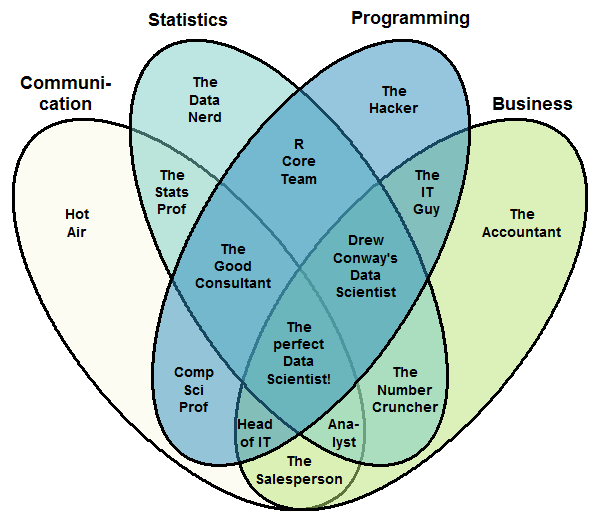
\includegraphics[height=0.8\textheight]{data_scientist}
	\end{figure}
\end{frame}

%------------------------------------------------

\begin{frame}
	\frametitle{Project}
	\begin{enumerate}
		\item Define a problem.
			\begin{itemize}
				\item Form groups.
				\item Write a proposal.
			\end{itemize}
		\vfill
		\item Solve it.
			\begin{itemize}
				\item Use the concepts learned in class.
				\item Follow the Data Science process.
			\end{itemize}
		\vfill
		\item Handle your solution for grading.
			\begin{itemize}
				\item Jupyter notebook as report.
				\item Oral presentation.
			\end{itemize}
	\end{enumerate}
\end{frame}

%------------------------------------------------

\begin{frame}
	\frametitle{Problem}
	\begin{center}
		Find a problem you want to solve.
	\end{center}
	\vfill
	%Sources of inspiration:
	\begin{itemize}
		\item Classic problems: Computer Vision, Natural Language Processing.
		\vfill
		\item Social websites are a wealth of information.\footnote{Not only
			Facebook and Twitter, but also GitHub, Pinterest, StackOverflow,
			YouTube, LinkedIn, Instagram, Tumblr, etc.}
		\vfill
		\item Your own interests: scientific, hobbies, or otherwise.
		\vfill
		\item Open challenges, e.g. \href{https://www.kaggle.com/}{kaggle} or \href{https://www.crowdai.org/}{crowdAI}.
		\vfill
		\item Any other.
		\vfill
		\item Discuss with us!
	\end{itemize}
\end{frame}

%------------------------------------------------

\begin{frame}
	\frametitle{Datasets}
	\begin{center}
		Some more ideas.
	\end{center}
	\vfill
	\begin{itemize}
		\item \href{https://github.com/mdeff/fma}{Free Music Archive (FMA)}
		\item \href{http://snap.stanford.edu/data/index.html}{Stanford Large Network Dataset Collection (SNAP)}
		\item \todo{We need more!}
		% Look at ADA and my list
	\end{itemize}
\end{frame}

%------------------------------------------------

\begin{frame}
	\frametitle{Data Science Process}
	\begin{figure}
		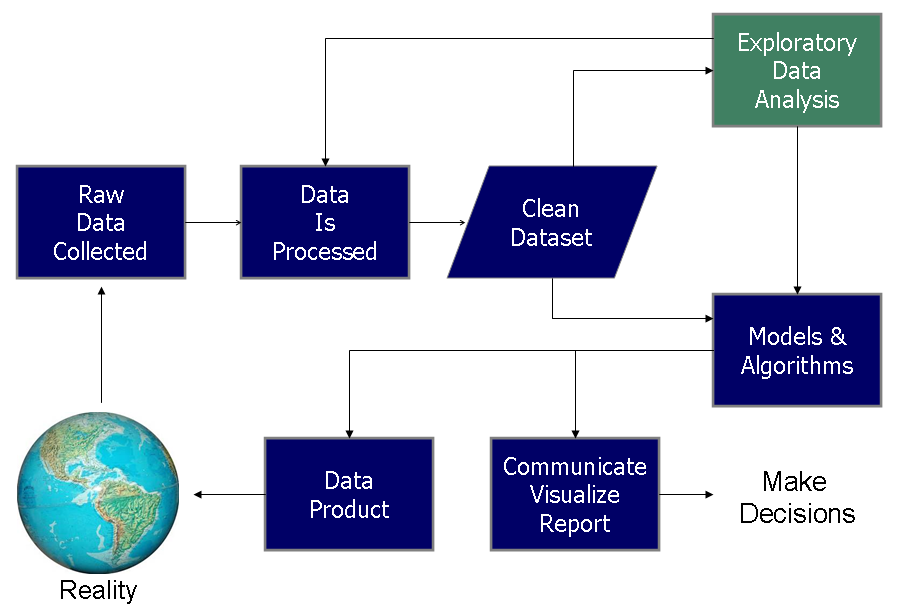
\includegraphics[width=\textwidth]{data_science_process}
	\end{figure}
\end{frame}

%------------------------------------------------

\begin{frame}
	\frametitle{Structure}
	The structure of the notebook will follow the Data Science process seen
	during the lab sessions.
	\vfill
	\begin{enumerate}
		\define{Data acquisition} from the web, a database, a flat file, etc.
			This includes cleaning the data.
		\vfill
		\define{Data exploration} some exploratory analysis to describe what
			you got. Very important to understand your data.
		\vfill
		\define{Data exploitation} use the data to draw conclusions.
			The concepts and algorithms taught in class must be used.
	\end{enumerate}
\end{frame}

%------------------------------------------------

\begin{frame}
	\frametitle{Practical aspects}
	\begin{itemize}
		\item Please isolate code blocks in functions and put those in a
			separate Python module.
		%\item Maximize the use of external libraries. You should invest time
			%in the problem, not in reinventing the wheel.
		\vfill
		\item Your notebook should be clean and legible. They are akin to a report.
		\vfill
		\item You can take inspirations from the notebooks seen during the
			lab sessions.
	\end{itemize}
\end{frame}

%------------------------------------------------

\begin{frame}
	\frametitle{Rules}
	\begin{itemize}
		\item The project includes graph and network data aspects, and more generally falls under the scope of the class.
		\vfill
		\item Form groups of 3 or 4 students. No less, no more.
			\begin{itemize}
				\item One member of the group uploads the deliverables.
				\item The names of all members should clearly appear.
			\end{itemize}
		\vfill
		\item The project should follow the data acquisition, exploration and exploitation workflow.
		\vfill
		\item Collecting data manually is optional, i.e. the use of datasets is allowed. \todo{Do we ask to compensate?}
		\vfill
		\item Each member will speak during the project presentation.
	\end{itemize}
\end{frame}

%------------------------------------------------

\begin{frame}
	\frametitle{Organization}
	\begin{enumerate}
		\define{Proposal} define the problem and explain your plan.
			\begin{itemize}
				\item Single page document.
				\item Organize yourselves in groups of three or four people.
				\item Deadline: Tuesday, November 28, 2017. Upload on Moodle.
				\item Not graded. Discussion with TAs will follow.
			\end{itemize}
		\vfill
		\define{Report} your solution, using the theory seen in class and the
			practical skills trained during labs.
			\begin{itemize}
				\item Jupyter notebook with text, math, code, analyzes and
					results.
				\item The notebook will be posted on the course git repository,
					on GitHub. You can use it for your portfolio!
				\item Deadline: Friday, January 12, 2017. Upload on Moodle.
				\item Graded.
			\end{itemize}
		\vfill
		\define{Presentation} impress us!
			\begin{itemize}
				\item Presentation of 15 minutes followed by 5 minutes of questions.
				\item Each group member must talk.
				\item Register for January 24 or 25 (once exams are scheduled).
				\item Graded.
			\end{itemize}
	\end{enumerate}
\end{frame}

\end{document}
